\documentclass[11pt,letterpaper]{article}

\usepackage[margin=1in]{geometry}
\usepackage{amsmath,amssymb}
\usepackage{mathtools}
\usepackage{booktabs}
\usepackage{enumitem}
\usepackage{hyperref}
\usepackage[dvipsnames]{xcolor}
\usepackage{titlesec}
\usepackage{microtype}
\usepackage{parskip}
\usepackage{array}
\usepackage{tikz}
\usetikzlibrary{arrows.meta,positioning}

\hypersetup{
  colorlinks=true,
  linkcolor=NavyBlue,
  citecolor=NavyBlue,
  urlcolor=NavyBlue,
  pdfstartview=FitH
}

\titleformat{\section}{\large\bfseries}{\thesection}{1em}{}
\titleformat{\subsection}{\normalsize\bfseries}{\thesubsection}{1em}{}
\titleformat{\subsubsection}{\normalsize\itshape}{\thesubsubsection}{1em}{}

\newcommand{\R}{\mathbb{R}}
\newcommand{\bz}{\mathbf{z}}
\newcommand{\bx}{\mathbf{x}}
\newcommand{\bp}{\mathbf{p}}
\newcommand{\bh}{\mathbf{h}}
\newcommand{\bs}{\mathbf{s}}
\newcommand{\bq}{\mathbf{q}}

\setlength{\emergencystretch}{3em}

\begin{document}

\begin{center}
{\LARGE\bfseries Neural Field Perceiver v14}\\[6pt]
{\large Phase-1 Architecture Spec for Cross-Patient Speech Decoding}\\[10pt]
{\normalsize Ben Tang \quad\textbar\quad Greg Cogan Lab, Duke University}\\[4pt]
{\normalsize April 2026 \quad\textbar\quad Internal design document}
\end{center}

\medskip\noindent\rule{\textwidth}{0.4pt}\medskip

\noindent
This document describes the active \textbf{Phase-1} v14 design only. It folds in the \textbf{B-1 amendment} of 2026-04-16 late, which replaced the per-parcel pooled-token interface with a per-electrode token interface plus a soft parcel embedding, and replaced factored spatial-then-temporal attention with combined spatiotemporal attention. The amendment record at \texttt{docs/v14\_core\_contract\_amendment\_2026-04-16.md} is the authoritative source for the rewrite rationale; the per-blocker status log at \texttt{docs/implementation\_tasks.md} remains the source of truth for implementation gating.


%% ====================================================================
\section{Problem and Scope}
%% ====================================================================

Each patient's $\mu$ECoG array is a sparse sample of cortical high-gamma activity during non-word repetition. Arrays are placed by the surgeon, not by protocol. Channel indices therefore have no shared meaning across patients.

Phase 1 asks one concrete question:
\begin{quote}
Can a fixed-atlas, shared model decode the 3-phoneme sequence of each trial across patients, using parcel identity as the only cross-patient anchor and without learned per-patient calibration?
\end{quote}

The task is the PhonemeSequence non-word repetition dataset:
\begin{itemize}[leftmargin=2em, itemsep=0.2em]
\item 52 canonical tokens, each 3 phonemes long
\item 9 phoneme classes (\texttt{AA, AE, B, G, IY, K, P, UW, V})
\item one sample = one response-onset-locked trial
\item input window: $t_{\min}=-0.5$\,s, $t_{\max}=1.0$\,s
\item signal: z-scored high-gamma at 200\,Hz
\end{itemize}

Phase-1 training and evaluation are \textbf{left hemisphere only}. Core patients are S14, S26, S33, and S62. Extended left-hemisphere patients S16, S23, and S39 audit in parallel. Right-hemisphere patients (S22, S58) and cross-modality joins are deferred to Phase 2.


%% ====================================================================
\section{Design Principle}
%% ====================================================================

v14 splits the problem into two parts:
\begin{enumerate}[leftmargin=2em, itemsep=0.2em]
\item \textbf{Spatial calibration} (per-patient, physics-constrained): patient-specific electrodes are placed in a shared atlas via a fixed Brainnetome surface parcellation on fsaverage. The atlas does $\approx 90\%$ of calibration; learned refinement is deferred to Phase 2.
\item \textbf{Shared dynamics} (cross-patient, unconstrained): a small relational-temporal transformer with an autoregressive decoder reads per-electrode tokens annotated with a soft parcel-identity embedding.
\end{enumerate}

The shared interface is a per-electrode token stream
\begin{equation}
\bz \in \R^{B \times (N_e \cdot T) \times d},
\end{equation}
with
\begin{itemize}[leftmargin=2em, itemsep=0.2em]
\item $N_e$ = patient-specific number of non-artifact electrodes (128 or 256 for the Phase-1 cohort)
\item $T = 28$ temporal tokens per trial (200\,Hz $\rightarrow$ 20\,Hz patches)
\item $d = 64$ by default, with $d=128$ as the first width ablation
\end{itemize}

Cross-patient sharing happens via a single learnable parcel-embedding lookup, not via per-parcel pooling. The lookup table has size $(15, d)$, where the 15 keys are the Tier-1 left-hemisphere Brainnetome parcels (\S\ref{sec:tier1}). $N_{\text{tok}} = 15$ is therefore the \emph{embedding-lookup table size}, not a token count.

Why this shape, and not the earlier $N_{\text{tok}} \times d \times T$ pooled interface? Three findings drove the rewrite:
\begin{enumerate}[leftmargin=2em, itemsep=0.2em]
\item \textbf{Vertex-collision audit (2026-04-16 late).} The strict fsaverage snap collides $\sim 23.6\%$ of electrodes per patient (302/1280 across 7 LH patients), with up to 4 electrodes mapped to the same vertex on the densest 128-channel grids. Per-parcel pooling cannot separate collided electrodes.
\item \textbf{$\mu$ECoG vs sEEG compression calculus.} A 15-token atlas pool compresses dense $\mu$ECoG by $22$--$30\times$ per active parcel, vs $\sim 5\times$ for sEEG. Sub-parcel somatotopy (Bouchard 2013, Conant 2018) sits at exactly the scale this pool would discard, and is what the dense device was meant to capture.
\item \textbf{Sub-parcel positional alignment is below the noise floor.} Registration noise ($\sim 3$--$5$\,mm RMS) plus inter-individual anatomical variability ($\sim 10$\,mm RMS) gives $\sim 11$\,mm joint uncertainty, while functional sub-parcel clusters are $5$--$10$\,mm wide. SNR for cross-patient sub-parcel positional alignment is $\le 1$. Any architecture that relies on aligning sub-parcel position across patients is fighting physics.
\end{enumerate}

The B-1 design respects all three: \emph{the rigid $\mu$ECoG grid is the spatial substrate, the parcel is the cross-patient anchor, and sub-parcel positional alignment is not encoded.}


%% ====================================================================
\section{Phase-1 Status}
%% ====================================================================

The Phase-1 contract is \textbf{fixed atlas, supervised only, no learned calibration}. Specifically:
\begin{itemize}[leftmargin=2em, itemsep=0.2em]
\item the Brainnetome PM volume at \texttt{data/atlas/BNA\_PM\_4D.nii.gz} is baked once onto fsaverage (per \#36)
\item patient electrodes project onto fsaverage via stock \texttt{sphere.reg} (snap-to-pial); the cvs\_avg35 cache from the cras-corrected Python port of Zac's \texttt{sub2AvgBrainClinical.m} is retained as a parity oracle only
\item no learned gain, offset, rigid correction, parcel offsets, or parcel temperatures
\item no MFA in the training path
\item no data augmentation in the first benchmark run
\item no SSL pretraining, no sEEG, no external datasets
\end{itemize}

\textbf{All Phase-1 blockers are closed} as of 2026-04-16 late. The two final closures were:
\begin{itemize}[leftmargin=2em, itemsep=0.2em]
\item \textbf{\#36} — fsaverage spatial pivot adopted after the cras-bug fix in the cvs\_avg35 oracle unblocked the parity comparison
\item \textbf{\#34} — phoneme loading audit closed across the full cohort; the \texttt{.fif} is the authoritative source for labels, response onsets, and signal, and the BIDS events TSV is a soft cross-check
\end{itemize}

The v14 loader is unblocked. The remaining work is execution against the frozen contract; the implementation order is in \texttt{docs/plans/v14-core.md}.


%% ====================================================================
\section{Model Overview}
%% ====================================================================

\begin{center}
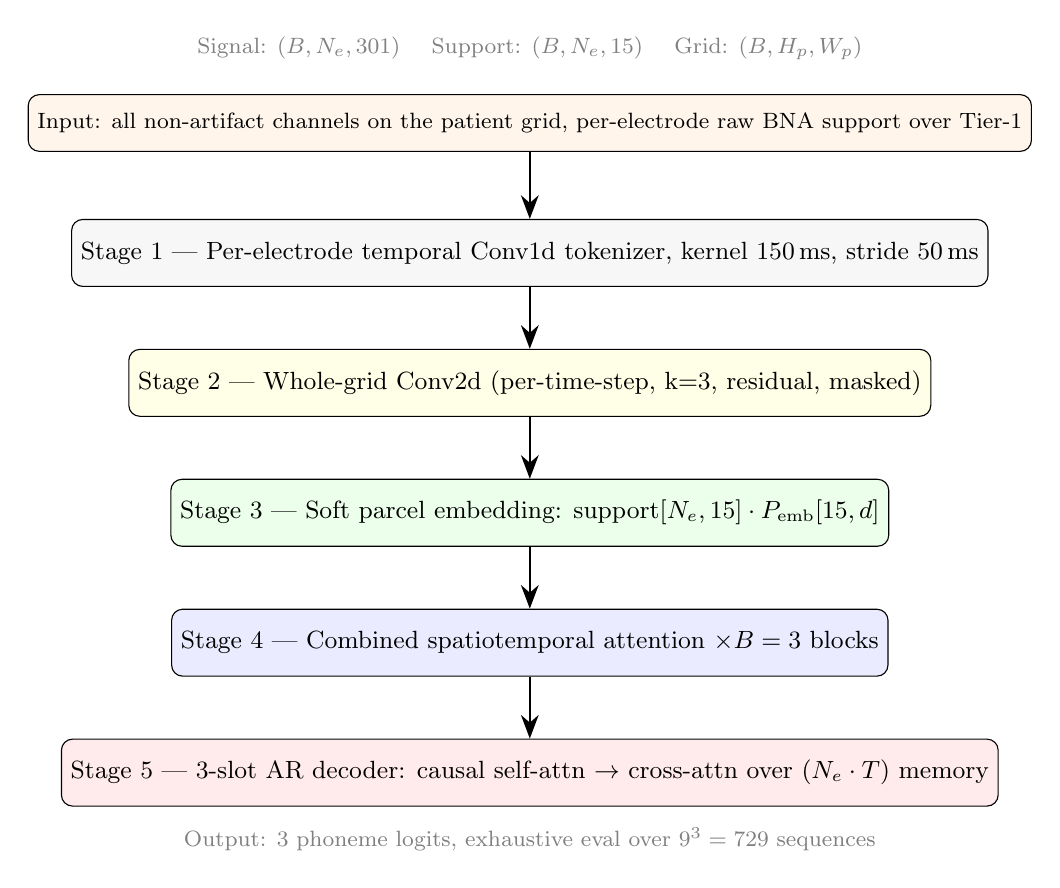
\begin{tikzpicture}[
  box/.style={draw, rounded corners, minimum width=8.4cm, minimum height=0.85cm, align=center, font=\small},
  smallbox/.style={draw, rounded corners, minimum width=8.4cm, minimum height=0.72cm, align=center, font=\footnotesize},
  arrow/.style={-{Stealth[length=3mm]}, thick}
]

\node[smallbox, fill=orange!8] (in) at (0, 4.6) {Input: all non-artifact channels on the patient grid, per-electrode raw BNA support over Tier-1};
\node[box, fill=gray!6] (tok) at (0, 2.95) {Stage 1 --- Per-electrode temporal Conv1d tokenizer, kernel 150\,ms, stride 50\,ms};
\node[box, fill=yellow!10] (mix) at (0, 1.3) {Stage 2 --- Whole-grid Conv2d (per-time-step, k=3, residual, masked)};
\node[box, fill=green!8] (sum) at (0, -0.35) {Stage 3 --- Soft parcel embedding: $\text{support}[N_e, 15] \cdot P_{\text{emb}}[15, d]$};
\node[box, fill=blue!8] (back) at (0, -2.0) {Stage 4 --- Combined spatiotemporal attention $\times B = 3$ blocks};
\node[box, fill=red!8] (dec) at (0, -3.65) {Stage 5 --- 3-slot AR decoder: causal self-attn $\rightarrow$ cross-attn over $(N_e \cdot T)$ memory};

\draw[arrow] (in) -- (tok);
\draw[arrow] (tok) -- (mix);
\draw[arrow] (mix) -- (sum);
\draw[arrow] (sum) -- (back);
\draw[arrow] (back) -- (dec);

\node[font=\footnotesize, text=gray] at (0, 5.55) {Signal: $(B, N_e, 301)$ \quad Support: $(B, N_e, 15)$ \quad Grid: $(B, H_p, W_p)$};
\node[font=\footnotesize, text=gray] at (0, -4.5) {Output: 3 phoneme logits, exhaustive eval over $9^3 = 729$ sequences};
\end{tikzpicture}
\end{center}

The architecture is intentionally small. Stage 1 extracts short local temporal features per electrode. Stage 2 mixes information across spatially adjacent electrodes on the patient grid. Stage 3 adds the cross-patient parcel-identity prior to each per-electrode token. Stage 4 models region-region and time-time interaction in a single combined attention. Stage 5 reads out a fixed 3-slot phoneme sequence.


%% ====================================================================
\section{Spatial Interface}
%% ====================================================================

\subsection{Coordinates and channel bridge}

The stable channel bridge ends at a physical electrode name. Under the fsaverage pivot (\#36), this name-keyed bridge terminates in a per-patient surface-projection cache
\begin{equation}
\texttt{data/fsaverage\_coords/<pt>\_fsaverage\_pial.csv},
\end{equation}
with the cvs\_avg35 MNI cache at \texttt{data/mni\_coords/<pt>\_MNI152.csv} retained as a parity oracle only. The lookup key is the \emph{physical electrode name} (concatenated from \texttt{<pt>.electrodeNames}), not a row index and not a TSV electrode name.

The channel bridge is:
\begin{equation}
\texttt{.fif channel} \rightarrow \texttt{amp channel} \rightarrow \texttt{layout map}
\rightarrow \texttt{physical electrode name} \rightarrow \texttt{fsaverage vertex} \rightarrow \texttt{support row}.
\end{equation}

The mapping is layout-specific:
\begin{itemize}[leftmargin=2em, itemsep=0.2em]
\item 128-strip patients (S14, S16, S22, S23, S26) use Map 4 from local \texttt{*\_channelMap.mat}
\item 256-grid patients (S33, S39, S62) use Map 3 from \texttt{*\_channelMapAll.mat}
\item S58 uses a cropped Map-3 variant aligned back to the full Map 3
\item the stray \texttt{S39\_channelMap.mat} is non-authoritative and must never be loaded
\end{itemize}

The bridge contract is frozen (per blocker \#12). The patient-by-patient verifier (Phase A2 in \texttt{docs/plans/v14-core.md}) also recovers the $(\text{row}, \text{col})$ of each electrode on the device grid, which Stage 2 needs to scatter onto the per-patient bounding rectangle.

\subsection{Patient-side vs atlas-side surfaces}

The two sides of the fsaverage pipeline use different surfaces:
\begin{itemize}[leftmargin=2em, itemsep=0.2em]
\item \textbf{Patient side}: project electrodes from each patient's \texttt{pial-outer-smoothed} surface through stock \texttt{sphere.reg} to fsaverage and snap to the nearest \texttt{lh.pial} vertex. This matches the physical fact that the electrodes sit on the dural envelope rather than on the cortical ribbon itself.
\item \textbf{Atlas side}: bake the Brainnetome PM volume through the true cortical ribbon, from \texttt{white} to \texttt{pial}, using \texttt{mri\_vol2surf --projfrac-avg 0 1 0.1} from \texttt{ICBM152\_fs}, then \texttt{mri\_surf2surf} to fsaverage, then 2D geodesic surface smoothing at FWHM 3.5\,mm. Output cache: \texttt{data/atlas/fsaverage\_bake\_fast2/}.
\end{itemize}

The PSF is baked into the atlas at bake time. There is no extra query-time Gaussian. Convolving again would double-smooth. The old nearest-neighbor 8\,mm dilation bridge belongs to the retired cvs\_avg35 path and is not part of the v14 spatial design.

\texttt{ICBM152\_fs} is not the atlas. It is the FreeSurfer reconstruction of the ICBM152 template, which provides white/pial surfaces in the same space as the BNA PM volume before the nonlinear \texttt{sphere.reg}-based transfer to fsaverage.

\subsection{Channel inclusion}

The input channel policy (per blocker \#11) is:
\begin{itemize}[leftmargin=2em, itemsep=0.2em]
\item use \textbf{all non-artifact channels}; do not silently filter to significant channels
\item remove artifact channels from the active channel axis; do not zero them in place
\item significant-channel masks are an ablation-only filter, not the default
\end{itemize}

\subsection{Tier-1 parcels}
\label{sec:tier1}

Phase 1 uses 15 fixed left-hemisphere Brainnetome parcels, derived 2026-04-16 late on the fsaverage bake under the frozen rule
\begin{equation}
\texttt{argmax\_wins}(p) \ge 10,
\end{equation}
where $\texttt{argmax\_wins}(p)$ is the number of Phase-1 LH electrodes for which $p$ is the dominant parcel across all 246 BNA ROIs. The cohort is 7 LH patients (S14, S16, S23, S26, S33, S39, S62), 1280 electrodes; the ranking source is \texttt{data/atlas/fsaverage\_parity/fsaverage\_cohort\_ranking.csv}. The argmax band $[5, 9]$ is empty, so any threshold in $[5, 10]$ yields the same 15 parcels.

The canonical list (and BNA 1-based indices) lives at \texttt{src/speech\_decoding/v14/token\_spec.DEFAULT\_BASE\_PARCELS}:
\begin{quote}
\texttt{A4hf, A1/2/3ulhf, A1/2/3tonIa, A4tl, IFJ, A44d, A45c, A6cvl, A9/46v, A40rd, IFS, A2, A40rv, A44v, A22r}.
\end{quote}

These 15 parcels span face/head and tongue M1/S1, ventral premotor, Broca (dorsal/caudal/ventral), inferior frontal sulcus and junction, supramarginal (rostrodorsal/rostroventral), area 2 (dorsal S1), and rostral area 22. Under B-1 they serve as the \textbf{embedding-lookup keys} for $P_{\text{emb}}$, not as fixed token slots.

\subsection{Support and validity}

Per-electrode parcel support is read directly from the baked atlas at the electrode's assigned fsaverage pial vertex (per blocker \#5):
\begin{equation}
\text{support}(e,p) = \texttt{fsaverage\_bake}[v_e, p],
\end{equation}
where $v_e$ is the fsaverage \texttt{lh.pial} vertex assigned to electrode $e$ by \texttt{src/speech\_decoding/v14/fsaverage\_projection.py}. Values are raw BNA probabilities (0--100), not row-normalized.

The full $(N_e, 15)$ support matrix is materialized once via \texttt{data/atlas/support\_cache/<pt>\_support\_tier1.csv} (Phase A1) and emitted by the loader directly. Electrode validity is \textbf{soft} (per blocker \#3 amended): support enters as a routing weight, not as a hard membership test. The only hard exclusion is \#11 (artifact channels). An electrode whose $\max_{p \in \text{Tier-1}} \text{support}(e,p) = 0$ is still emitted, but its parcel-embedding contribution is zero by construction.

\subsection{Loader contract}

The v14-core sample dict (per blocker \#13 amended) is:
\begin{equation*}
\begin{array}{lll}
\texttt{signal}                  & \in \R^{N_e \times 301}      & \text{float32, productionZscore HGA, 200\,Hz, 1.5\,s} \\
\texttt{patient\_id}             & \in \text{str}               & \text{e.g. ``S14''} \\
\texttt{label}                   & \in \{0,\ldots,8\}^{3}        & \text{0-indexed alphabetical ARPABET} \\
\texttt{electrode\_grid\_layout} & \in \mathbb{Z}^{N_e \times 2} & (\text{row}, \text{col}) \text{ on patient grid} \\
\texttt{electrode\_grid\_shape}  & = (H_p, W_p)                  & \text{per-patient bounding rect} \\
\texttt{electrode\_active\_mask} & \in \{0,1\}^{N_e}             & \text{non-artifact and not pad} \\
\texttt{support}                 & \in \R^{N_e \times 15}        & \text{raw BNA probability over Tier-1}
\end{array}
\end{equation*}

The fields \texttt{coords[N\_ch, 3]}, \texttt{token\_mask[N\_tok]}, and \texttt{token\_support[N\_tok]} from the pre-amendment contract are removed. There are no per-parcel tokens, so per-parcel masks are irrelevant; spatial-coordinate PE is dropped because the Conv2d (Stage 2) already encodes local position and that position is not patient-transferable.


%% ====================================================================
\section{Stage 1 --- Temporal Tokenizer}
%% ====================================================================

The temporal front-end is per-electrode, shared across all patients (per blockers \#2, \#6):
\begin{equation}
\bx \in \R^{B \times N_e \times 301}
\;\rightarrow\;
\bh \in \R^{B \times N_e \times d \times 28}.
\end{equation}

For each electrode independently, apply a shared Conv1d patch projection:
\begin{itemize}[leftmargin=2em, itemsep=0.2em]
\item input rate: 200\,Hz
\item input channels: 1, output channels: $d = 64$
\item kernel: 150\,ms = 30 samples
\item stride: 50\,ms = 10 samples
\item bias: True
\item temporal compression: $10.7\times$, matching the HGA envelope timescale
\end{itemize}

Output rate is 20\,Hz, giving $T = 28$ patches per 1.5\,s window. The token semantics are overlapping temporal patches, not continuous framewise states. There is no spatial mixing in Stage 1.


%% ====================================================================
\section{Stage 2 --- Whole-Grid Conv2d}
%% ====================================================================

Stage 2 mixes information across spatially adjacent electrodes on the rigid $\mu$ECoG grid. The output of Stage 1 is scattered onto the per-patient bounding rectangle:
\begin{equation}
\bh \in \R^{B \times N_e \times d \times T}
\;\xrightarrow{\text{scatter}}\;
\bx \in \R^{B \times d \times H_p \times W_p \times T},
\end{equation}
with a per-cell active mask in $\{0,1\}^{B \times H_p \times W_p}$ (false on pad cells and on artifact channels). Per-patient bounding rectangles are e.g.\ $H_p \times W_p = 8 \times 16$ for S14, $16 \times 16$ for S33, $12 \times 24$ for S58.

Per time step, with weights shared across $t$:
\begin{align}
\bx_{\text{normed}} &= \operatorname{LayerNorm}_{\text{channel}}(\bx) \\
\bx_{\text{conv}}   &= \operatorname{GELU}\!\left(\operatorname{Conv2d}(\bx_{\text{normed}})\right) \\
\bx_{\text{out}}    &= \bx + \bx_{\text{conv}} \odot \text{active\_mask}
\end{align}
with kernel $3\times3$, stride 1, padding 1, full channel mixing, pre-norm LayerNorm, residual masked by the active mask. The default depth is one layer; depth 2 is ablation A3.

Justifications:
\begin{itemize}[leftmargin=2em, itemsep=0.2em]
\item \textbf{Receptive field.} A $3\times3$ kernel covers $\pm 1.33$--$3$\,mm at typical $\mu$ECoG pitch, which matches the HGA spatial correlation length.
\item \textbf{Full channel mixing.} $64 \times 64 \times 9 \approx 37$K parameters per layer is trivial at our scale; depthwise-separable saves nothing.
\item \textbf{Per-time-step.} Temporal mixing belongs to Stage 4. Stage 2 is a pure spatial mixer.
\item \textbf{Mask handling.} Pad cells and artifact channels are zeroed from the residual contribution, so they do not bleed through the conv.
\end{itemize}

After Stage 2, gather back to the per-electrode layout: $(B, d, H_p, W_p, T) \rightarrow (B, N_e, d, T)$.


%% ====================================================================
\section{Stage 3 --- Soft Parcel Embedding}
%% ====================================================================

Stage 3 adds the only cross-patient anatomical signal in the model. For each electrode $e$, the parcel-identity contribution is a support-weighted sum over a learnable lookup table:
\begin{equation}
\text{parcel\_emb}(e) = \sum_{p \in \text{Tier-1}} \text{support}(e, p) \cdot P_{\text{emb}}[p],
\qquad
P_{\text{emb}} \in \R^{15 \times d}.
\end{equation}
$P_{\text{emb}}$ is Xavier-uniform initialized and has zero per-patient parameters. Support is consumed raw (not row-normalized), so electrodes outside Tier-1 contribute weak embeddings naturally and electrodes split across two parcels get a convex-like combination of both embeddings.

The Stage-3 token, broadcast across time, is:
\begin{equation}
\text{token}(e, t) = \bh_{\text{conv}}(e, t) + \text{parcel\_emb}(e).
\end{equation}

Flatten to the backbone input:
\begin{equation}
\bz \in \R^{B \times (N_e \cdot T) \times d},
\qquad
\text{token\_active\_mask} \in \{0,1\}^{B \times (N_e \cdot T)},
\end{equation}
where the active mask is \texttt{electrode\_active\_mask} broadcast across $T$.

What this token deliberately contains:
\begin{itemize}[leftmargin=2em, itemsep=0.2em]
\item sub-parcel functional information: implicit in $\bh_{\text{conv}}$ via Stage 2 grid mixing
\item parcel identity: explicit via the soft $\text{parcel\_emb}$, the cross-patient anchor
\item boundary-awareness: a convex combination for electrodes that straddle two Tier-1 parcels
\end{itemize}

What it deliberately does not contain:
\begin{itemize}[leftmargin=2em, itemsep=0.2em]
\item grid-coordinate embedding (Stage 2 already encodes local position; not transferable across patients)
\item intra-parcel coordinate (PE-2 / PE-3 / parcel frames) --- registration noise dominates anatomical variability, so cross-patient sub-parcel alignment is below the SNR floor
\item fsaverage vertex coordinate --- collision-prone and not transferable
\item hard parcel argmax --- replaced by soft probability weighting
\end{itemize}

The within-parcel Perceiver summarizer (the pre-amendment design) is retired. The parcel-frame chart and \texttt{parcel\_frames.npz} are retired. The mean+gradient pool is the main linear ablation (A5), not a pipeline element.


%% ====================================================================
\section{Stage 4 --- Combined Spatiotemporal Backbone}
%% ====================================================================

After Stage 3 the model operates on a single per-electrode token stream:
\begin{equation}
\bz \in \R^{B \times (N_e \cdot T) \times d},
\qquad N_e \in \{128, 256\}, \; T = 28.
\end{equation}

The backbone is $B = 3$ \textbf{combined} attention blocks. Each block is one combined-attention layer over all $(N_e \cdot T)$ tokens, followed by an FFN:
\begin{align}
\bq &= \operatorname{LayerNorm}(\bz) \\
\bz &\leftarrow \bz + \operatorname{MultiHeadAttention}(\bq, \bq, \bq;\, \text{mask}, \text{RoPE}_{\text{temp}}) \\
\bz &\leftarrow \bz + \operatorname{FFN}(\operatorname{LayerNorm}(\bz))
\end{align}

Hyperparameters:
\begin{itemize}[leftmargin=2em, itemsep=0.2em]
\item $\text{num\_heads} = 4$, $\text{head\_dim} = 16$ (so $\text{num\_heads} \cdot \text{head\_dim} = d = 64$)
\item FFN: \texttt{Linear}$(d \rightarrow 4d) \rightarrow \operatorname{GELU} \rightarrow \texttt{Linear}(4d \rightarrow d)$, hidden width $4d = 256$
\item pre-norm, dropout 0.1
\item RoPE on the temporal axis only: rotation depends on $t_a - t_b$ and is identity for token pairs at the same $t$
\item attention mask: \texttt{token\_active\_mask} broadcast to pairs, applied on both key and query axes
\item inactive query rows zeroed after each block (storage hygiene; the mask carries the semantics)
\end{itemize}

Why combined and not factored:
\begin{itemize}[leftmargin=2em, itemsep=0.2em]
\item \textbf{Compute is not binding.} At the worst-case 256-channel patient, $N_e \cdot T = 7168$ tokens, combined attention is $\sim 13$\,B FLOPs per layer and $\sim 80$\,B per forward, well within budget.
\item \textbf{Combined captures lag-coupled cross-region patterns in one layer.} Speech production has planning $\rightarrow$ execution $\rightarrow$ feedback patterns that are intrinsically cross-spatial-temporal. Factored attention requires a 2-layer composition to express the same $(e_i, t_a) \rightarrow (e_j, t_b)$ interaction.
\item \textbf{$B = 3$ blocks (down from 6 factored half-blocks).} Each combined block is more expressive, fewer are needed.
\item \textbf{No spatial PE.} Spatial relationships emerge from data plus the soft parcel embedding plus the Stage 2 conv. The temporal axis is the only one with an explicit positional prior.
\end{itemize}

\textbf{No SC/FC bias in the baseline.} The structural- and functional-connectivity additive logit bias (originally in \#8) is deferred to ablation A4. When reintroduced it will be per-(layer, head) learnable scalars $\alpha_{\text{SC}}, \alpha_{\text{FC}}$ over a precomputed $\text{support} \cdot \text{SC}_{\text{norm}} \cdot \text{support}^\top$ parcel-pair bias, broadcast across temporal pairs.

The full $(N_e \cdot T, d)$ backbone output is handed to the decoder. There is no early pooling.


%% ====================================================================
\section{Stage 5 --- Decoder and Supervision}
%% ====================================================================

The target is a fixed 3-slot phoneme sequence over the 9 canonical ARPABET classes, alphabetically indexed (per blocker \#16):
\begin{equation}
\texttt{AA}=0,\;
\texttt{AE}=1,\;
\texttt{B}=2,\;
\texttt{G}=3,\;
\texttt{IY}=4,\;
\texttt{K}=5,\;
\texttt{P}=6,\;
\texttt{UW}=7,\;
\texttt{V}=8.
\end{equation}

The decoder (per blocker \#28) is one small autoregressive block:
\begin{itemize}[leftmargin=2em, itemsep=0.2em]
\item one learned base query, plus one slot embedding per position (3 slots)
\item previous-token embedding injected into the query stream
\item one causal self-attention layer across the 3 slots
\item one cross-attention layer over the flattened backbone memory $M \in \R^{(N_e \cdot T) \times d}$
\item one shared linear vocab head
\end{itemize}

Slot $k$ computes
\begin{equation}
q'_k = q_k + \operatorname{emb}(y_{k-1}),
\qquad
u_k = \operatorname{CausalSelfAttn}(q'_k),
\qquad
o_k = \operatorname{CrossAttn}(u_k, M),
\qquad
\hat{y}_k = W o_k.
\end{equation}

Cross-attention naturally handles the variable $N_e \cdot T$ memory size across patients.

\subsection{Loss and decode}

The baseline supervised loss is plain slot-wise cross-entropy (per blocker \#9):
\begin{equation}
\mathcal{L} = \frac{1}{3}\sum_{k=1}^{3} \operatorname{CE}(\hat{y}_k, y_k).
\end{equation}

There is no label smoothing, focal loss, mixup, or auxiliary token head in the first benchmark run. Training uses teacher forcing.

Evaluation uses exhaustive decoding over all $9^3 = 729$ possible sequences. Greedy decoding is allowed as a comparison path only. The reported metric is slot-averaged phoneme error rate (PER).


%% ====================================================================
\section{Hyperparameter Summary}
%% ====================================================================

\begin{center}
\small
\begin{tabular}{@{}p{3.4cm} p{4.0cm} p{7.6cm}@{}}
\toprule
\textbf{Stage} & \textbf{Field} & \textbf{Value} \\
\midrule
Stage 1 (Conv1d) & in/out channels & 1 / 64 \\
                 & kernel / stride & 30 samples (150\,ms) / 10 samples (50\,ms) \\
                 & output rate     & 20\,Hz, $T = 28$ \\
\midrule
Stage 2 (Conv2d) & in/out channels & 64 / 64 \\
                 & kernel / stride / pad & 3 / 1 / 1 \\
                 & channel mixing  & full \\
                 & num\_layers     & 1 (depth 2 = ablation A3) \\
                 & norm / activation & pre-norm LayerNorm / GELU \\
                 & residual        & masked by \texttt{electrode\_active\_mask} \\
\midrule
Stage 3 (Embed)  & $P_{\text{emb}}$ shape & $(15, 64)$ \\
                 & init             & Xavier uniform \\
                 & support          & raw (not normalized) \\
                 & Tier-1 source    & \texttt{token\_spec.DEFAULT\_BASE\_PARCELS} \\
\midrule
Stage 4 (Backbone) & num\_blocks    & 3 \\
                 & $d_{\text{model}}$ & 64 (128 = ablation A1) \\
                 & num\_heads / head\_dim & 4 / 16 \\
                 & FFN width / activation & 256 = $4d$ / GELU \\
                 & norm / dropout   & pre-norm LayerNorm / 0.1 \\
                 & attention        & combined spatiotemporal \\
                 & RoPE axis        & temporal only \\
                 & SC/FC bias       & none in baseline (ablation A4) \\
\midrule
Stage 5 (Decoder) & num\_slots      & 3 \\
                 & self-attn / cross-attn layers & 1 / 1 \\
                 & vocab head       & shared linear, 9 phonemes \\
                 & training / eval  & teacher-forced / exhaustive $9^3$ \\
\bottomrule
\end{tabular}
\end{center}


%% ====================================================================
\section{Training and Evaluation Defaults}
%% ====================================================================

These are not architecture innovations. They are frozen first-run defaults chosen to prevent protocol drift.

\subsection{Evaluation}

\begin{itemize}[leftmargin=2em, itemsep=0.2em]
\item grouped-by-token cross-validation (per blocker \#33)
\item 5 outer folds
\item 3 seeds: 42, 137, 256
\item 20\% grouped validation split within each training fold
\item same train/val partition reused across seeds within fold
\item report per-patient PER mean $\pm$ std across seeds, then population mean
\end{itemize}

\subsection{Training}

\begin{itemize}[leftmargin=2em, itemsep=0.2em]
\item optimizer: AdamW
\item base learning rate: $10^{-3}$
\item weight decay: $10^{-4}$
\item scheduler: cosine decay
\item warmup: 20 epochs
\item gradient clipping: 1.0
\item mixed precision on by default on DCC unless unstable
\item early stopping on validation PER
\end{itemize}

\subsection{Batching}

\begin{itemize}[leftmargin=2em, itemsep=0.2em]
\item grouped-by-patient batches (per blocker \#31)
\item baseline run is per-patient first
\item \texttt{trials\_per\_batch = 8}
\item effective batch target 32 via gradient accumulation if needed
\item max epochs 300
\item patience 10 validation checks
\item validation every 5 epochs
\end{itemize}


%% ====================================================================
\section{Ablation Plan}
%% ====================================================================

Once \texttt{v14-core} is running and overfits a tiny subset cleanly, the following ablations execute in priority order (Phase F):
\begin{enumerate}[leftmargin=2em, itemsep=0.2em]
\item \textbf{A3 (depth-2 GridMixer)} --- Stage 2 \texttt{num\_layers = 2}
\item \textbf{A1 ($d_{\text{model}} = 128$)} --- width sweep
\item \textbf{A2 (block count)} --- $B \in \{2, 4\}$ vs $B = 3$ baseline
\item \textbf{A4 (SC/FC bias)} --- per-(layer, head) $\alpha_{\text{SC}}, \alpha_{\text{FC}}$ over a parcel-pair bias
\item \textbf{A5 (mean+gradient linear pool)} --- main linear comparator to the soft embedding
\item \textbf{A6 (factored attention head-to-head)} --- factored as historical reference
\item \textbf{A7 (intra-parcel PE-2)} --- patient-grid bbox PE; tests whether explicit position helps despite the alignment-noise argument
\end{enumerate}


%% ====================================================================
\section{What Is Deferred}
%% ====================================================================

The following are explicitly not part of the Phase-1 base architecture:
\begin{itemize}[leftmargin=2em, itemsep=0.2em]
\item learned per-patient calibration ($\Delta/\omega$, $\delta_l$, $\tau_l$, additional gain/offset)
\item SSL pretraining
\item sEEG
\item right-hemisphere integration (S22, S58)
\item external datasets (Flinker, Chang chronic ECoG)
\item broad recipe ablations (label smoothing, focal loss, mixup, augmentation)
\item articulatory or auxiliary heads
\end{itemize}

For future external datasets with uncertain MNI quality, a reasonable Phase-2 fallback is:
\begin{enumerate}[leftmargin=2em, itemsep=0.2em]
\item freeze the shared neural network weights
\item fit a per-patient rigid-body coordinate adapter only
\item restrict that adapter to rotation plus translation, not free affine warping
\end{enumerate}

That should be treated as an explicit external-dataset adaptation step, not as part of the base Phase-1 contract.


%% ====================================================================
\section{Sequencing}
%% ====================================================================

\begin{itemize}[leftmargin=2em, itemsep=0.2em]
\item \textbf{Phase 1}: supervised \texttt{v14-core} on response-locked $\mu$ECoG, 4 core LH patients, 5 folds $\times$ 3 seeds = 60 jobs on DCC
\item \textbf{Phase 1.5}: SSL on the full continuous $\mu$ECoG corpus (not response-locked-only)
\item \textbf{Phase 2}: learned per-patient calibration on top of the fixed-atlas baseline
\item \textbf{Phase 3+}: sEEG join, external datasets, broader scaling
\end{itemize}

The current state is: all blockers closed, the contract is frozen, and the work is implementation against \texttt{docs/plans/v14-core.md}. Performance against the historical $0.734 \pm 0.007$ S14 baseline is the next conversation, after correctness lands.


\small
\begin{thebibliography}{99}\raggedright
\setlength{\itemsep}{2pt}

\bibitem{duraivel2023}
Duraivel, S., et al.\ (2023).
High-resolution neural recordings improve the accuracy of speech decoding.
\textit{Nature Communications}, 14, 6938.

\bibitem{fan2016}
Fan, L., et al.\ (2016).
The Human Brainnetome Atlas.
\textit{Cerebral Cortex}, 26(8), 3508--3526.

\bibitem{bouchard2013}
Bouchard, K. E., Mesgarani, N., Johnson, K., \& Chang, E. F.\ (2013).
Functional organization of human sensorimotor cortex for speech articulation.
\textit{Nature}, 495(7441), 327--332.

\bibitem{conant2018}
Conant, D. F., Bouchard, K. E., Leonard, M. K., \& Chang, E. F.\ (2018).
Human sensorimotor cortex control of directly measured vocal tract movements during vowel production.
\textit{Journal of Neuroscience}, 38(12), 2955--2966.

\bibitem{spalding2025}
Spalding, Z., et al.\ (2025).
Cross-patient speech decoding from intra-operative $\mu$ECoG.
(In preparation.)

\bibitem{oganesian2025}
Oganesian, L., et al.\ (2025).
BarISTA: parcel-embedding architectures for cross-patient intracranial decoding.

\end{thebibliography}

\end{document}
